\documentclass[t]{beamer}
\usetheme{hkllite}

\title{Advanced regression}
	\author{François Briatte, Ivaylo Petev \& Joël Gombin}
	\date{Week~\#10}

\graphicspath{{images/}}

\begin{document}
    

    \frame[plain]{
        \titlepage\\[7em]
        \tableofcontents[hideallsubsections]
        }

    
		
		


	\begin{frame}[c]%{Multiple linear regression}
			
		\begin{center}
			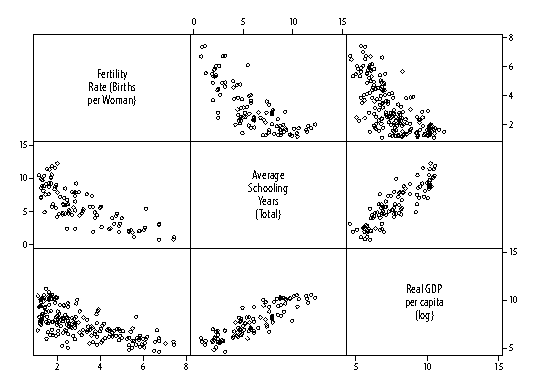
\includegraphics[width=\textwidth]{mreg-gr-mat.pdf}
		\end{center}
				
	\end{frame}

    \section{Multiple linear regression}

	
	\begin{frame}[c]{Multiple linear regression} % or, as my girlfriend calls it, ultimate regression
			
		\begin{center}
			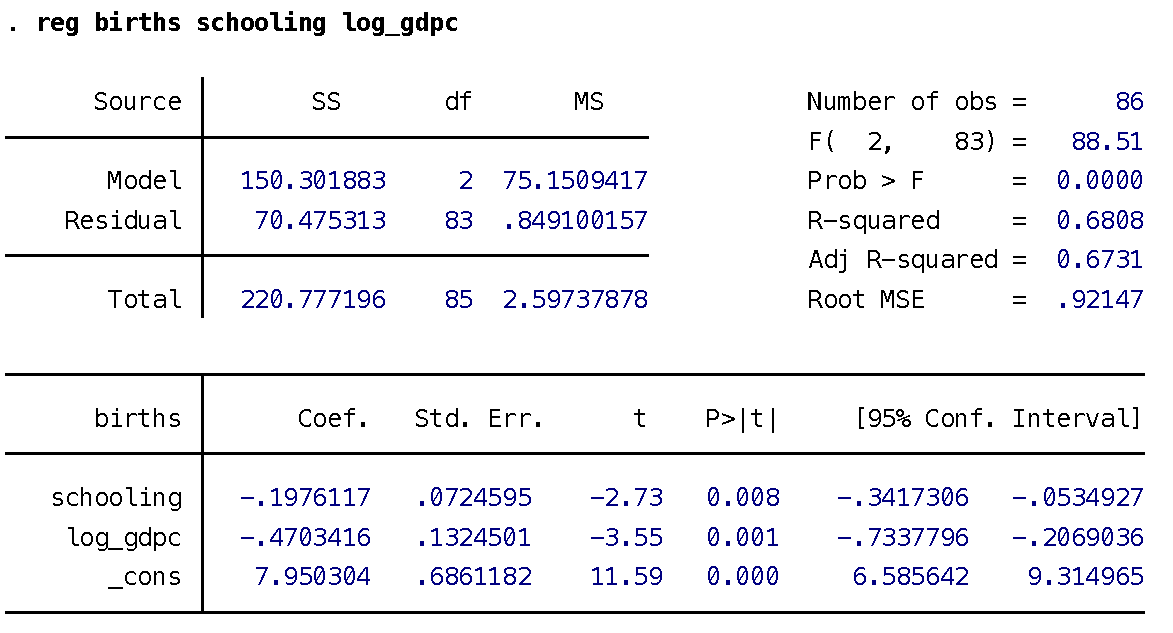
\includegraphics[width=\textwidth]{mreg-output.pdf}
		\end{center}
				
	\end{frame}	

	\begin{frame}[c]{Multiple linear regression}
		
		$$Y = \alpha+\beta_1 X_1+\beta_2 X_2+,\ldots,+\beta_k X_k+\epsilon$$
		
		\vfill
		 
		\begin{block}{Partial derivatives}

			Each coefficient is calculated by \red{holding all others constant}.

		\end{block}

		\begin{block}{Least squares}

			The model is still optimized by minimizing the squared error terms.

		\end{block}

		\begin{alertblock}{Sanity check}

			The model is still assuming \emph{linear}, \emph{additive} relationships.

		\end{alertblock}
				
	\end{frame}


	\begin{frame}[c]{Logarithmic coefficients: see \href{http://www.ats.ucla.edu/stat/mult_pkg/faq/general/log_transformed_regression.htm}{UCLA mini-guide}}
	
		\begin{block}{Linear-linear relationships: $Y = \alpha + \beta_1 X$}
			An increase of one unit of $X$ is associated with an increase of $\beta_1$ units of $Y$.
		\end{block}
	
		\begin{block}{Log-linear relationships: $\red{\ln Y} = \alpha + \beta_1 X$}
			An increase of one unit of $X$ is associated with a $100 \times \beta_1$\% increase in $Y$ (true effect: $Y \times$ \texttt{exp($\beta_1$)}).
		\end{block}

		\begin{block}{Linear-log relationships: $Y = \alpha + \red{\beta_1 \ln X}$}
			A 1\% increase in $X$ is associated with a $0.01 \times \beta_1$ unit increase in $Y$ (e.g. $\beta_1 \times$ \texttt{log(1.15)} for +15\% in $X$).
		\end{block}
	
		\begin{block}{Log-log relationships: $\red{\ln Y} = \alpha + \red{\beta_1 \ln X}$}
			A 1\% increase in $X$ is associated with a $\beta_1$\% increase in $Y$.
		\end{block}
	
	\end{frame}
	
		\section{Standardized coefficients}

	\begin{frame}[t]{\texttt{reg births schooling log\_gdpc\red{, beta}}}

%		Each variable can be normalized to fit $\mathcal{D} \sim \mathcal{N}(0,1)$, so that their \red{standardized coefficients} have comparable standard deviation units:
		Each variable can be normalized to have a mean of 0 and a standard deviation of 1, so that their \red{standardized coefficients} have comparable standard deviation units:
		
		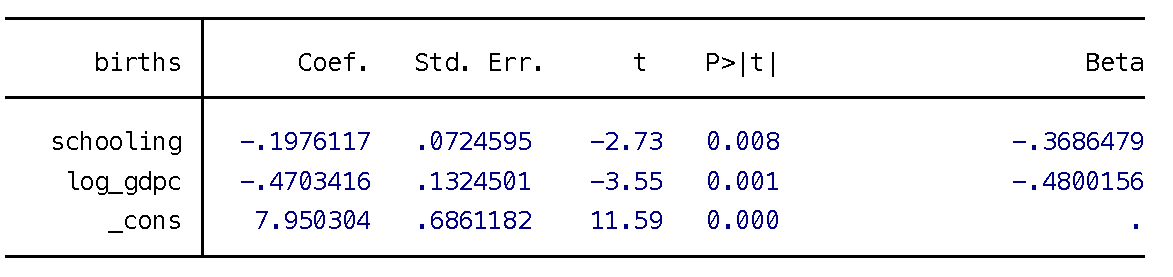
\includegraphics[scale=.45]{mreg-output-beta.pdf}

		\footnotesize{\textit{(identical output for overall model fit omitted)}}
		
		\begin{alertblock}{Sanity check}

			Interpret unstandardized coefficients; use standardization only for model comparisons.

		\end{alertblock}

	\end{frame}

		\section{Regression dummies}

		\begin{frame}[t]{Regression dummies and categorical predictors}

			\begin{block}{Single coefficient of dummy $X_3$}

				\vspace{-1em}
				\begin{align*}
					Y &= \alpha + \beta_1 X_1 + \beta_2 X_2 + \color{gray} \beta_3 (0) \color{fg} + \epsilon \\
					Y &= \alpha + \beta_1 X_1 + \beta_2 X_2 + \red{\beta_3 (1)} + \epsilon
				\end{align*}

				The omitted category $X_3 = 0$ is called the \red{reference category} and is part of the \red{baseline model} $Y = \alpha$, for which all coefficients are null.
				
			\end{block}
			
			\begin{exampleblock}{Example}

				\vspace{-1em}
				\begin{align*}			
					Income &= \alpha + \beta_1 \cdot \text{age} + \beta_2 \cdot \text{education} + \color{gray} 0 \cdot \text{male} \color{fg} & + \epsilon \\
					Income &= \alpha + \beta_1 \cdot \text{age} + \beta_2 \cdot \text{education} + \red{1 \cdot \text{female}} & + \epsilon
				\end{align*}

			\end{exampleblock}
			
		\end{frame}
					
	\begin{frame}[t]{\texttt{reg births schooling log\_gdpc \red{i.region}}}

		Categorical variables can be used as \red{dummies}, i.e. binary recodes of each category that are tested against a \red{reference category} to provide regression coefficients for the net effect of each category:\\[.5em]

		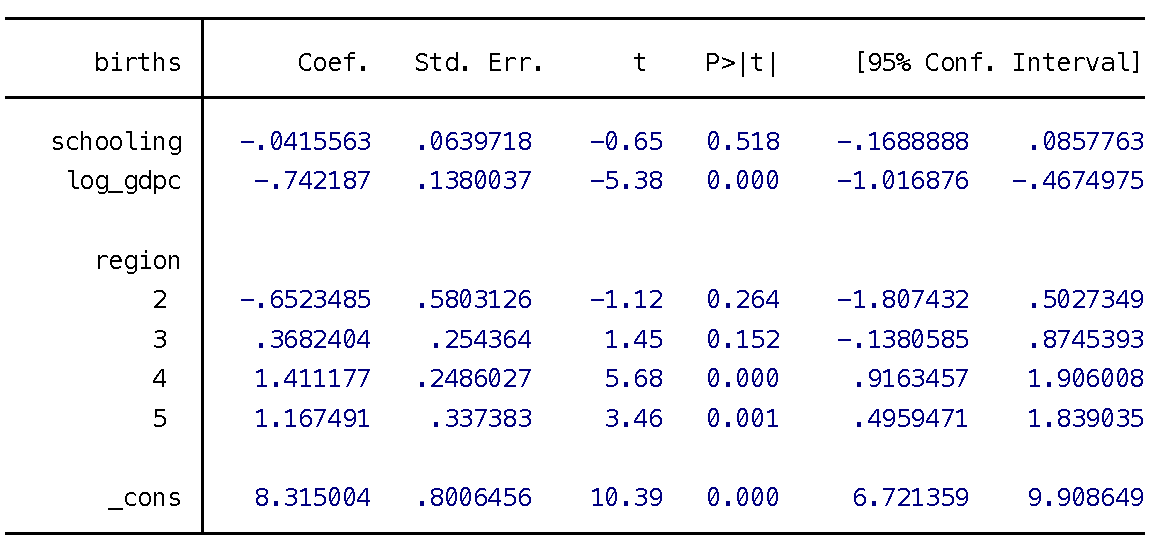
\includegraphics[scale=.45]{mreg-output-dummies.pdf}

		\footnotesize{\textit{(identical output for overall model fit omitted)}}

	\end{frame}

	\section{Regression diagnostics}

	\begin{frame}[t]{Regression diagnostics}

		\begin{block}{Residuals}

			\begin{itemize}
				\item \texttt{predict yhat}: fitted values
				\item \texttt{predict r, resid}: residuals
				\item \texttt{predict r, rsta}: standardized residuals		
			\end{itemize}
			
			Use \texttt{rvfplot} for residuals-versus-fitted values plots.

		\end{block}

		\begin{alertblock}{Heteroskedasticity}

			When the residuals are not normally distributed, the model expresses \red{heterogeneous variance} (unreliable standard errors).

		\end{alertblock}

		\begin{exampleblock}{Examples: \href{http://www.ats.ucla.edu/stat/stata/webbooks/reg/chapter2/statareg2.htm}{UCLA \textit{Regression with Stata}, ch.~2}}

			There are many more diagnostics on display there.

		\end{exampleblock}
		
	\end{frame}

    %
    %
    	
	\begin{frame}[t]{Regression diagnostics}

		\begin{block}{Interaction terms}

			\begin{itemize}
				\item Use \texttt{\#} and \texttt{\#\#} to capture interactions
				\item Use \texttt{c.} to interact continuous variables
			\end{itemize}
			
			(See also \texttt{avplot} and partial regression.)
		\end{block}

		\begin{alertblock}{Variance inflation}

			Variables that strongly interact induce \red{multicollinearity} `inside' your model, making standard errors unreliable and coefficient estimates unstable.
			\begin{itemize}
				\item 	 Use \texttt{vif} to detect variables with $VIF > 10$
			\end{itemize}
			


		\end{alertblock}

		\begin{exampleblock}{Examples: \href{http://www.ats.ucla.edu/stat/stata/faq/}{UCLA Stata FAQ}}

			Search for ``comparing coefficients across groups''.

		\end{exampleblock}
					
	\end{frame}

\section{Logistic regressions}

	\begin{frame}[t]{Outline}
	
	\begin{block}{Equations}
	
	$$\text{Linear model:~} Y = \beta_0 + \beta_1 X_1 + \beta_2 X_2 + \epsilon$$
	$$\text{Logistic model:~} Pr(Y=1) = \frac{exp(\beta_0 + \beta_1 X_1 + \beta_2 X_2 + \epsilon)}{1+exp(\beta_0 + \beta_1 X_1 + \beta_2 X_2 + \epsilon)}$$
	\end{block}
		
	\red{Bivariate statistics} look at the probability of an association between two variables and are part of \red{inferential statistics}.\\[.5em]
	

	\end{frame}
	
	
	
	

	\subsection{Odds ratios}

	\begin{frame}[t]{\red{Odds ratios}}
					
		\begin{quote}
		``Scotland has 13\% redheads, Kabylie has 4\% redheads.''\\
		``Scots are \red{more likely} to be redheads than Kabyles.''
		\end{quote}
		
		Quantify the second statement.

		\begin{itemize}
			\item \textbf{Treat the dependent variable as a binary `success/failure':}\\1 is success (red hair), 0 is failure (other colour).
						
			$$\textsf{Odds of \textit{p}:~}\frac{\textsf{red hair}}{\textsf{other colour}}=\frac{p}{1-p}=\frac{\textsf{success}}{\textsf{failure}}$$
			\vspace{0em}
			
			\item \textbf{Divide the odds in each group to compare across them:} the odds ratio quantifies their comparative likelihood of success.
			
			$$\theta = \frac{\textsf{odds}_{\textsf{Scotland}}}{\textsf{odds}_{\textsf{Kabylie}}}=\frac{\textsf{odds}_1}{\textsf{odds}_2}=\frac{\textsf{success}_1}{\textsf{failure}_1}\times\frac{\textsf{failure}_2}{\textsf{success}_2}$$
						
		\end{itemize}

	\end{frame}
	
	\subsubsection{Computation}

	\begin{frame}[t]{Comparison with \red{odds ratios}}
					
		\begin{quote}
		``Scotland has 13\% redheads, Kabylie has 4\% redheads.''\\
		``Scots are \red{more likely} to be redheads than Kabyles.''
		\end{quote}
		
		Quantify the second statement.
		
		\begin{columns}[t]
		\column{.55\textwidth}
		\vspace{-.5em}
		% \begin{center}
		% \begin{tabular}{lcc}
		% 	\toprule
		% 	& \multicolumn{2}{c}{Hair colour} \\
		% 	\cmidrule(r){2-3}
		% 	Population & Red & Other \\
		% 	\midrule
		% 	Scotland & .13 & $1-.13=.87$\\
		% 	Kabylie & .04 & $1-.04=.96$ \\
		% 	\bottomrule
		% \end{tabular}\\[0em]
		% \end{center}
		
		\column{.25\textwidth}
		\vspace{3.275em}	
		$$\hspace{-3em}\theta = \frac{.13}{.87}\times\frac{.96}{.04}\approx\red{3.5}$$
		\end{columns}
	
	\vspace{1.5em}
	Scots are roughly \red{3.5 times more likely} to have red hair than Kabyles. (\href{http://en.wikipedia.org/wiki/Red_hair}{All figures taken from current Wikipedia estimates.})
		
	\end{frame}	

\begin{frame}[t]{Logit regression}
    A logit model takes as dependant variable the log odds of $Y$.   
\vspace{3.275em}

For an example, see: \url{http://www.ats.ucla.edu/stat/stata/dae/logit.htm}
\vspace{3.275em}

Stata command: (surprisingly) \texttt{logit}
\vspace{3.275em}

The \texttt{or} option computes odd ratios instead of coefficients. 

\end{frame}

	\begin{frame}[t]{Practice session}

    \begin{block}{Class}
      \comm{Get the do-file for this week.}\\
      \code{srqm\_get week10bis.do}\\
      
			\comm{Open to read and replicate.}\\
			\code{doedit code/week10bis}\\    
    \end{block}

    \begin{alertblock}{Coursework}
      \begin{itemize}
	       \item Finish the do-file and read all comments at home.
	       \item Follow instructions on top of the code.
      \end{itemize}
    \end{alertblock}
    		
	\end{frame}
    
\end{document}